\documentclass[conference]{IEEEtran}
\usepackage{graphicx}
\usepackage{lipsum}
\usepackage{cite}
% *** MATH PACKAGES ***
\usepackage{amsmath}
% *** SPECIALIZED LIST PACKAGES ***
\usepackage{algorithmic}
% *** ALIGNMENT PACKAGES ***
\usepackage{makecell}
\usepackage{array}
\usepackage{float}
\usepackage[utf8x]{inputenc}
\usepackage{gensymb}

\makeatletter
\def\endthebibliography{%
  \def\@noitemerr{\@latex@warning{Empty `thebibliography' environment}}%
  \endlist
}
\makeatother

\author{
    \IEEEauthorblockN{Shashank Reddy Boosi\IEEEauthorrefmark{1}, David Sison\IEEEauthorrefmark{1}, Harmanpreet Singh\IEEEauthorrefmark{1}, Aravind Murugesan\IEEEauthorrefmark{1}, Allen kombasseril\IEEEauthorrefmark{1}}
    \IEEEauthorblockA{\IEEEauthorrefmark{1} School of Computing\\   { { University of New South Wales}}
    \\\{z5222766, z5019783, z5228917, z5175965, z5232188\}@student.unsw.edu.au}
}

\begin{document}

\title{Automation of Diabetic Lesions and blood vessels using Unet and Gaussian Pyramids}


% make the title area
\maketitle

% As a general rule, do not put math, special symbols or citations
% in the abstract
\begin{abstract}
 \textbf{\textit{Task 1}} - Diabetic retinopathy, known as diabetic eye disease, is a medical condition which damages the retina due to diabetes mellitus. This report is an attempt to solve the problem where we use Deep Learning to segment the four categories of lesions in a retinal image. We present a network and training strategy that relies on the strong use of data augmentation to use the available annotated samples efficiently. The architecture consists of a contracting path to capture context and a symmetric expanding path that enables precise localization. The model used is a fine tuned U-Net which is an enhanced encoder-decoder CNN model and we attained Jaccard Similarity of 0.3093 and a Dice Similarity of 0.3838 respectively.


\par
\setlength{\parskip}{1em}
\setlength{\parindent}{0em}

\textbf{\textit{Task 2}} - The segmentation of blood vessels can be used for various retinal imaging. We present a report of our study of a Resolution Hierarchy based method. The method reduces computational needs and could detect vessel of different thickness by using a Gaussian resolution hierarchy. The algorithm reported an accuracy of 87.5\% while taking less time to run. 

\paragraph*{Keywords}
Diabetic Retinopathy, Blood Vessels, UNet, Gaussian Pyramid.

\end{abstract}

% no keywords



% For peer review papers, you can put extra information on the cover
% page as needed:
% \ifCLASSOPTIONpeerreview
% \begin{center} \bfseries EDICS Category: 3-BBND \end{center}
% \fi
%
% For peerreview papers, this IEEEtran command inserts a page break and
% creates the second title. It will be ignored for other modes.
\IEEEpeerreviewmaketitle

\section{Task 1}

\subsection{Introduction}
\par
Diabetic retinopathy, a chronic, progressive eye disease, has turned out to be one of the most common causes of vision impairment and blindness especially for working ages in the world today\cite{1}. Retinal abnormal conditions are associated with lesions namely microaneurysms, haemorrhages, hard exudates and soft exudates. The diagnosis in the early stages of the disease is particularly important to receive proper treatment and reduce the chance of progression of the disease to advanced stages which can lead to permanent loss of vision in extreme cases\cite{2}. The presence of these lesions is highly correlated with DR, so detection of their presence is crucial. Retinopathy detection system is usually accomplished by involving a well-trained physician manually detecting vascular abnormalities and structural changes of retina in the retinal fundus images. These results are closely observed by expert readers but they often inconsistent as the method is manual in nature\cite{8}. So an automated method is necessary to identify these defects. 
\par
Most of the problems of computer vision of recent times have been solved with great accuracy with the help of modern deep learning algorithms, Convolutional Neural Networks (CNN's) to name one. Here we are using a tweaked version of the Fully connected convolutional neural network named UNET, which was developed by Olaf Ronneberger et al\cite{unet}, which have shown impressive results for biomedical image segmentation problems with lower number of training images.

\subsection{Related Works}
\par

Automatic diabetic retinopathy detection system can be achieved by various different algorithms and methods. Earlier solutions were based on hand-crafted feature extraction and standard machine learning algorithm for prediction\cite{3}. C.Sinthanayothin used Recursive region growing segmentation algorithms along with the use of a new technique , named as ‘Moat Operator’ to detect defects such as haemorrhages, microaneurysms and hard exudates. They ended up with a sensitivity and specificity for exudate detection of 88.5\% and 99.7\% respectively . They could detect microaneurysms, haemorrhages with a sensitivity and specificity of 88.7\% and 77.5\% respectively. 

\par

Sheikh Muhammad Saiful Islam used Deep learning methods along with data preprocessing and data augmentation for Early Detection and Grading of Diabetic Retinopathy\cite{8}. Their network achieved 98\% sensitivity and more than 94\% specificity in early-stage detection and on the challenging Kaggle EyePACS dataset\cite{9}.
\par

There was also a challenge\cite{idrid} hosted on Grand Challenges in Biomedical Imaging Platform.. One of the challenges in this competition was mainly to segment the lesions in a retinal image. For lesion segmentation task, most of the participating teams used U-Net architecture\cite{unet}. Unsurprisingly, the best approach for lesion segmentation in this competition used U-Net, with data augmentation boosting results significantly. It resulted in AUC of 0.8263, 0.9716, 0.9540 and 0.9883 for MA, HE, SE and EX respectively. 
\par
Olaf Ronneberger demonstrated the application of the U-NET to three different segmentation tasks\cite{unet}. One of it was a cell segmentation task in light microscopic images. This segmentation task is part of the ISBI cell tracking challenge 2014 and 2015\cite{6, 7}. Here they achieved an average IOU (Intersection over Union) of 92\%.
\par
This motivated us to use U-Net for the given task.


\subsection{Methodology}                                                                     
Fig. \ref{fig:dl} shows us an overview of the methodology pipeline. Our methodology consists of various steps: Image augmentation, Image pre-processing, and Modelling where we start with preparing the dataset, augmenting using selective resampling, preprocessing, fine tuning the model, training and testing. The data-set is taken from IDRiD Grand Challenge \cite{idrid}. We mainly  used imgaug, opencv and pytorch\cite{torch} and pandas library for all the steps involved in the methodology. Section \ref{sssec:describe} to section \ref{paragraph:metrics} consist of detailed information of the steps.    
\par              
\begin{figure*}[t]
	\centering
	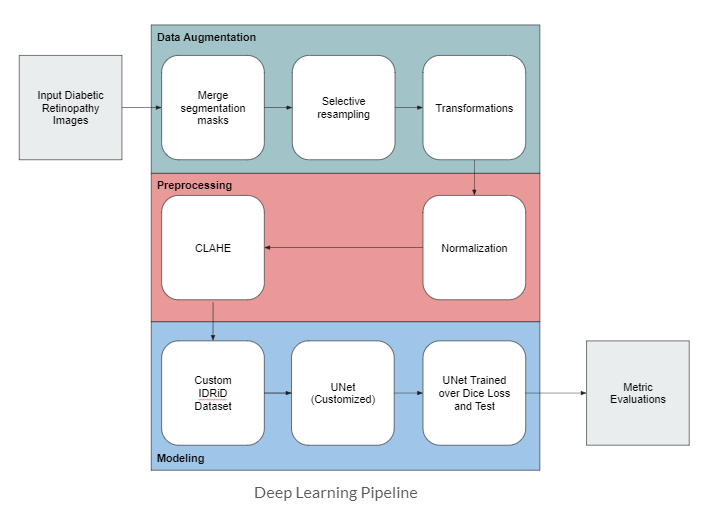
\includegraphics[scale=0.7]{image/dl_pipeline.PNG}
	\caption{Deep Learning Pipeline Overview}
	\label{fig:dl}
\end{figure*}

\subsubsection{Data Description}
\label{sssec:describe}
We have a total of 54 train images and 27 test images which is a multi class segmentation problem. 
\par
The input images contains the 3 channel retina and the label images contain 4 images of 1 channel diabetic lesions namely Microaneurysms, Haemorrhages, Hard Exudates and Soft Exudates per every input image.

\subsubsection{Merge Segmentation masks}
\label{sssec:merge}

A single segmentation mask was generated from the available segmentation masks per image by stacking binary masks across an axis and taking the argmax per pixel. This resulted in integer encoding of the 4 categories of the lesions and the background.
\begin{itemize}
		\item \textbf{0}  - Background
		\item \textbf{1}  - Haemorrhages
		\item \textbf{2}  - Hard exudates
		\item \textbf{3}  - Microaneurysms 
  		\item \textbf{4}  - Soft Exudates
\end{itemize} 



\subsubsection{Image Augmentation}
\label{sssec:aug}
Data augmentation is essential to teach the network the desired invariance and robustness properties, when only few training samples are available. After generating the segmentation masks, it was found that there was a huge imbalance between the background data and the other categories. To counter this, using visual cues and masks’ histograms, 16 images were selected to augment the data in the following way, 

\begin{itemize}
		\item \textbf{Crop} Images were cropped from the left and right sides to remove background.
		\item \textbf{Geometric} Randomly apply 
					\begin{enumerate}
  						\item Rotation between $0^{0}$ to $360^{0}$
	  					 \item Shear with angle between $-20^{0}$ and $20^{0}$
  					 	\item Flip horizontal or vertical
  					 	\item Shift images between −25 and 25 pixel
  					 	\item Zoom image on a random scale
					\end{enumerate}
		\item Finally, images(including the original) were partitioned into 4 parts and resized to 256x256
\end{itemize} 

\subsubsection{Image preprocessing}
\label{sssec:preprocess}

Due to different Lighting conditions and capture setup of the images , these images suffer a lot of  exposure and lighting variation. To normalize these effects we subtracted our local average colour as shown in  fig \ref{fig:pre} first image. The result obtained was further processed using contrast limited adaptive histogram equalization(CLAHE) as shown in fig \ref{fig:pre} second image. This is a special technique in which we increase the local contrast of the image without amplifying any noise in the image . This is a modified version of Adaptive Histogram equalization(AHE) where they limit amplification to not over amplify any noise like how CLAHE would. The resultant image obtained after these two steps are visibly enhanced to bring out the lesions to be segmented.

\par              
\begin{figure}[H]
	\centering
	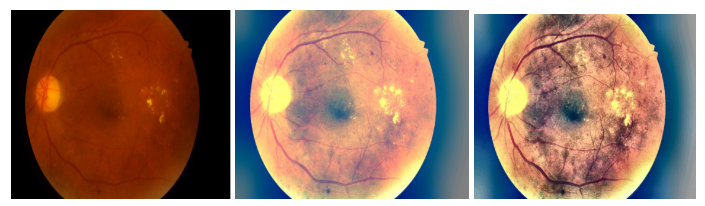
\includegraphics[width=\linewidth]{image/preprocess.PNG}
	\caption{Augmented Image to Normalization to CLAHE}
	\label{fig:pre}
\end{figure}

\subsubsection{UNet Modelling}
\label{sssec:model}

\begin{itemize}
\item After the preprocessing is done  we feed the images to the customized pytorch IDRiD dataset which will return us a dictionary images of the dimension \par 
		\textbf{Images}: (B, C, H, W)        \textbf{Masks}: (B, H , W)
\item We will split the dataset to train and validation with 20 percent being the validation.
\item  We have 940 train and 236 test images and then feed it to the customized UNet model.
\item \textbf{Model Details}
					\begin{itemize}
					\item \textbf{Optimizer} Adam 
					\item \textbf{Learning Rate} 0.01 
					\item \textbf{Loss} Dice Loss
					\end{itemize}
\end{itemize}

U-Net\cite{unet} is a convolutional neural network that was developed for biomedical image segmentation which is a fully convolutional network. It is a U- shaped architecture which is famous for its upsampling part (decoder) and usage is the skip connection which are introduced in Resnet\cite{res} from the downsampling part to the upsampling part which will help it to store the features from the down sampling as it helps to resize the image in an efficient manner. Fig \ref{fig:unet}  shows the traditional UNet architecture.

\par              
\begin{figure}[H]
	\centering
	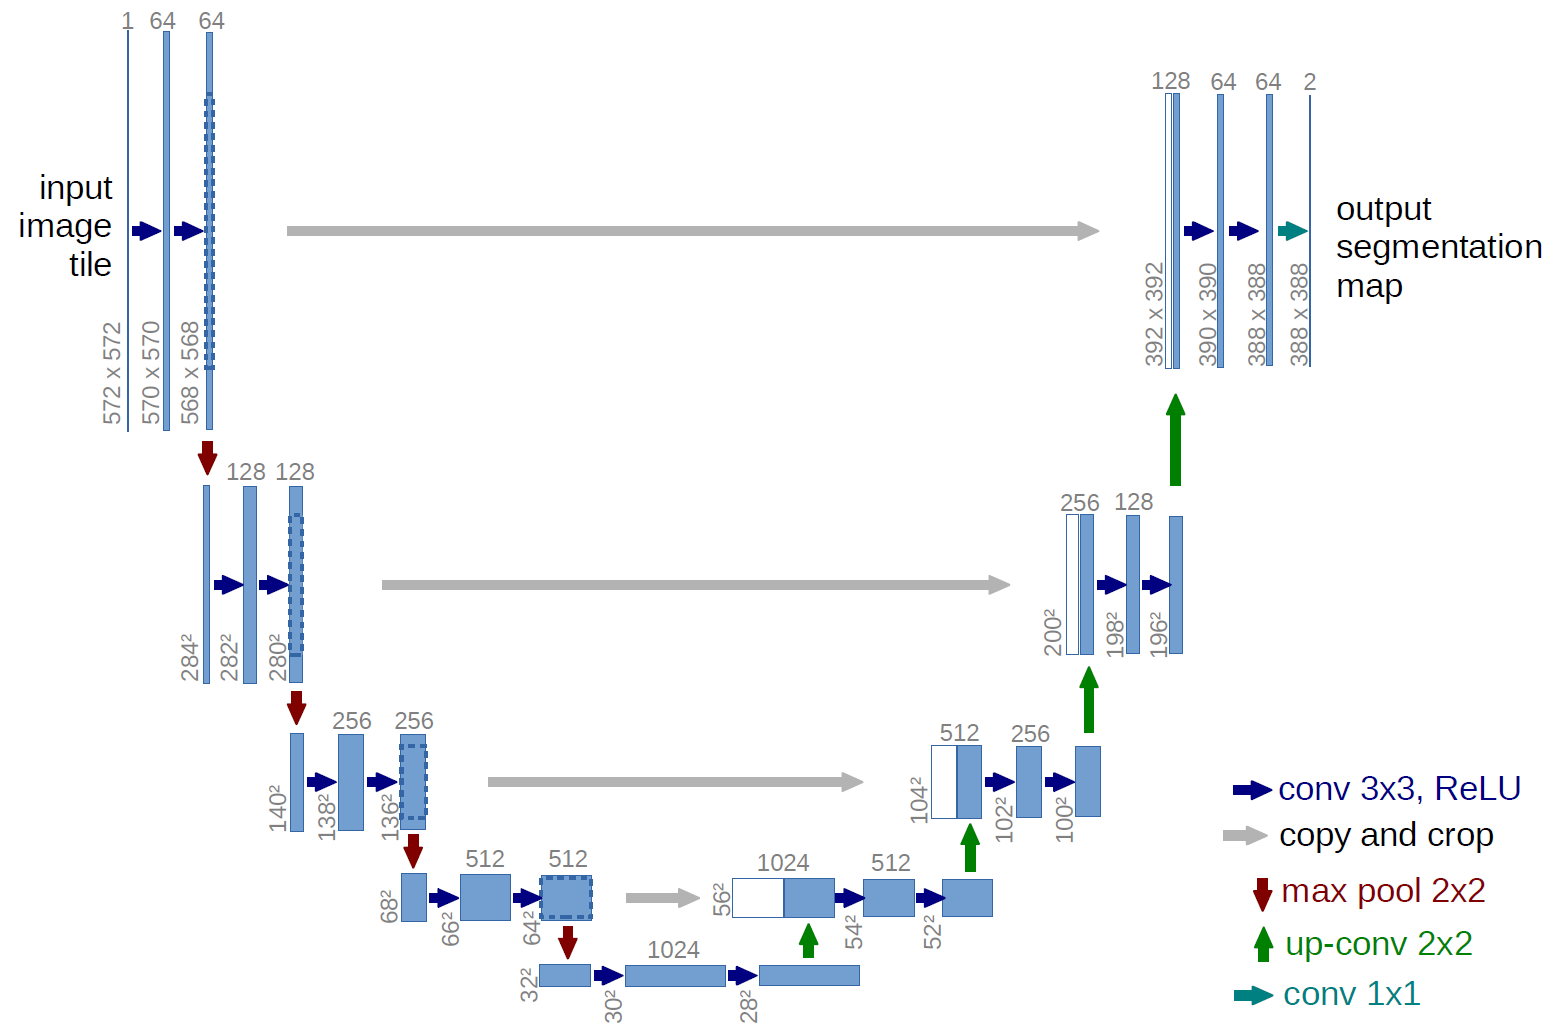
\includegraphics[width=\linewidth]{image/unet.PNG}
	\caption{UNet Architecture}
	\label{fig:unet}
\end{figure}

\par 
As the input and the output dimensions of the UNet are not of the same dimension we fine tuned the UNet and customized it to return a dimension which is the same as input for us to compare with the label. Fig \ref{fig:unetcustom} custom Unet below is an example of the customized UNet architecture.

\par              
\begin{figure}[H]
	\centering
	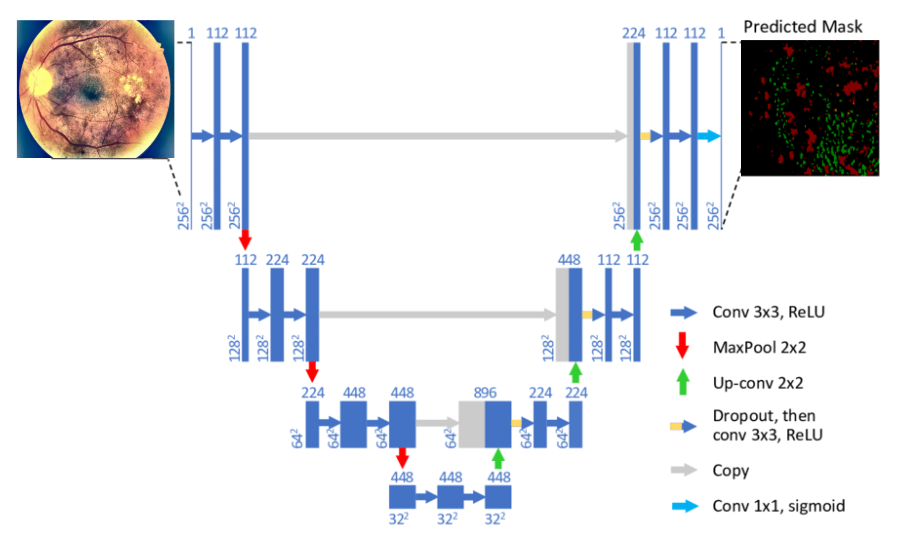
\includegraphics[width=\linewidth]{image/customunet.PNG}
	\caption{Customized UNet Architecture}
	\label{fig:unetcustom}
\end{figure}


\subsubsection{Experiment Setup}
\label{sssec:setup}

The network architecture of our U-net is shown in Fig \ref{fig:unet}. In deep networks with many convolutional layers and different paths through the network, a good initialization of the weights is extremely important. Hence, we used Xavier initialization. It works because we want the variance of the input to be as the variance of the output.
\par 
Batch Normalization was added as it not only result in faster training but also helps to reduce the sensitivity to the initial starting weights.
\par
Dropout was added at the bottleneck as it reduces the tendency for the model to overfit by providing a form of regularization.
\par
The network was trained with Adam with a fixed schedule over 50 epochs. The learning rate for Adam was gradually changed from 0.0001 to 0.01 as the loss function was converging very slowly. To fit the model in our GPU memory (3 GB), we reduce the batch to a single image of size 256x256.
\par
For hyper-parameter optimization, we used a random search over the respective ranges by running a few epochs (5 or 10) with cross validation.
\par
To train the network, cross entropy loss function was used initially, but the results were pretty ordinary. We believe it is because of the class imbalance present in the original input data. We experimented with weighted cross entropy but setting up the weights for this task turned out to be difficult with minimal to no improvement in results. Finally, a resampling strategy was devised to counter this and the loss function was changed to soft dice which is better at handling such cases.

\paragraph{Metrics}
\label{paragraph:metrics}
The combination of all the steps are evaluated under different performance metrics, including accuracy, accuracy per class, Jaccard Similarity Coefficient, Dice Similarity Coefficient for the multi class Segmentation. The metrics are defined as following,

\begin{equation}
JSC = \frac{|S \cap T|}{|S \cup T|} = \frac{|TP|}{|TP| + |FP| + |FN|}
\end{equation}

\begin{equation}
DSC = 2\frac{|S \cap T|}{|S| + |T|} = \frac{2|TP|}{2|TP| + |FP| + |FN|}
\end{equation}

\begin{equation}
Accuracy = \frac{1}{n}\sum\limits_{i=1}^{n} \frac{|X_i \cap Y_i|}{|X_i \cup Y_i|}
\end{equation}

where $TP$ is the true positive, $FP$ is the False Positive, $FN$ is the False Negative, $X_i$ is the set of predicted labels, $Y_i$ is the set of true labels and n is the number of samples.

\subsection{Evaluation and Results}
\label{sssec:results}

Table \ref{table:1} shows us the model performance in terms of metrics for UNet we have experimented. The metrics used for evaluation are overall accuracy, accuracy per class, Jaccard Similarity, Dice Similarity as shown in the section \ref{paragraph:metrics}. As we can see, the comparison between the train and test helped us understand the nature of how UNet is acting and predicting without over-fitting or under-fitting based on the metrics. The overall accuracy is just a measure to detect the whole image including the background but our goal is to detect the diabetic lesions without the background. So I used a metric called accuracy per class where every class used has a weight over the others. But the most famous metrics for semantic segmentation is the Jaccard Similarity and Dice similarity which will not include the background while only calculating the intersection over the union. Comparison between other papers is not done because most of the papers use the full dataset if IDRiD and comparing those papers with our implementation would not be fair.

\begin{table}[H]
\centering
 \begin{tabular}{|c| c c|} 
 \hline
 Metrics & Train & Test\\ [0.5ex] 
 \hline
 Overall Accuracy & 0.9460 & 0.9272\\ 
 \hline
 Accuracy per class & 0.4570 & 0.4130\\
 \hline
 Jaccard Similarity & 0.3431 & 0.3093\\
 \hline
 Dice Similarity & 0.4253 & 0.3838\\
 \hline
\end{tabular}
\vspace*{0.25cm}
\caption{Model Performance of UNet}
\label{table:1}
\end{table}

The main reason to get the Jaccard index of 0.3093 is because of the amount of data provided to us and the limited amount of features that can be obtained by the model. Another reason is the amount of background in every image is dominating the actual classes that we are detecting. Fig  \ref{fig:epoch} shows how the metrics are acting for each epoch.
              
\begin{figure}[H]
	\centering
	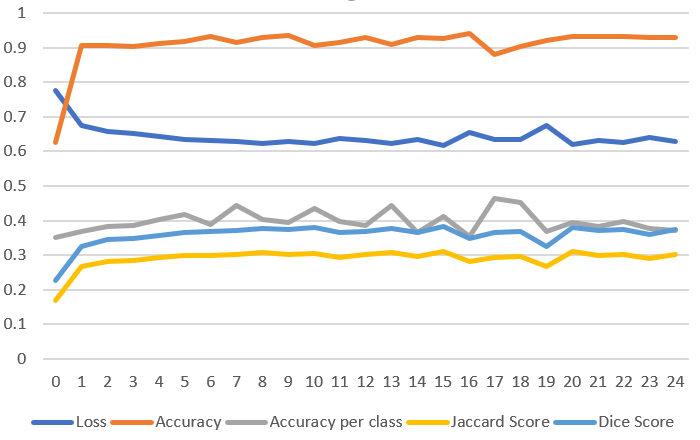
\includegraphics[width=\linewidth]{image/epochvsmetrics.PNG}
	\caption{Epoch vs Metrics Graph}
	\label{fig:epoch}
\end{figure}

Figure \ref{fig:good} and \ref{fig:bad} are the examples for the images with good predictions and the bad predictions. The main difference noticed between the  good and the bad predictions is that the images which has a good predictions contains a lot of diabetic lesions covered and for the bad predictions most of the image is covered with the background leading to the wrong prediction. We mitigated this effect by using a concept called selective resampling but removing this problem completely can only be done if we can increase our training data.

              
\begin{figure}[H]
	\centering
	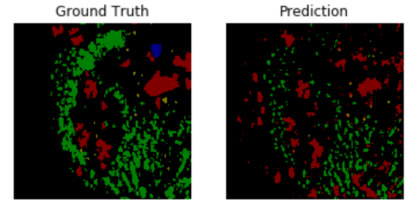
\includegraphics[width=\linewidth]{image/good.PNG}
	\caption{Image with good prediction}
	\label{fig:good}
\end{figure}
  
\begin{figure}[H]
	\centering
	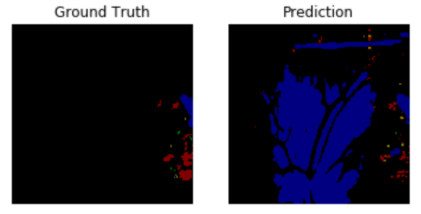
\includegraphics[width=\linewidth]{image/bad.PNG}
	\caption{Image with bad prediction}
	\label{fig:bad}
\end{figure}

\subsection{Conclusion and Future Work}
In this paper, the problem of summarizing UNet Deep Learning model which is used for retinal lesions associated with Diabetic Retinopathy in Augmented IDRiD datasets is discussed. The focus is mainly on using customized UNet to effectively segment the retinal lesions associzted with Diabetic Retinopathy \cite{monoclonal1} . For prediction we used an augmented dataset with 940 train images and 236 validation images and it is preprocessed to remove noise and contrasted with CLAHE. The outcome of the predictive results on the IDRiD data-set reveals the accuracy, accuracy per class, Jaccard Similarity Coefficient and Dice Similarity Coefficient with a score of 92.72, 41.30, 30.93, 38.38 \% respectively. The second conclusion gives us an intuition of how Dice loss performed better than the other loss functions like Binary cross entropy without weights, pixel wise cross entropy using weights.
\par 
The proposed work can be enhanced by expanding its scope to using Transfer Learning with pre trained models like Resnet 50, Resnet 101 or Inception v3. Hyper parameter Tuning the weights for the data imbalance will also improve the Pixel wise Cross Entropy Loss Function and finally we can use different type of Segmentation models like Residual nets, FCN etc.,


\section{Task 2}

\subsection{Introduction}
\par
Eye disease is one of the leading causes of blindness and can often be prevented by early detection. In common practice this is done by opthamologists by visual inspection alone, through the analysis of photos of the back of the eye taken using a fundus camera. Computer vision techniques can be used to speed up the process of diagnosis by trained professionals by automatically segmenting and tagging relevant regions of interest. In this task we aim to implement a segmentation algorithm to automatically and accurately segment the blood vessels in a fundus image.
\par
Although this problem, like many others within the image segmentation and classification fields, can be solved by using a convolutional neural network (CNN), we have decided to implement a standard segmentation algorithm instead. This is in part motivated by the desire to avoid a similar implementation to Task 1, but also by the results from implementations described in the papers from our literature review. We have been providing a total of 20 training images and 20 testing images, but as our algorithm requires no training we instead use all of them for testing.

\subsection{Related Works}
\par
Attila Budai, Georg Michelson, and Joachim Hornegger's paper "Multiscale Blood Vessel Segmentation in Retinal Fundus Images" \cite{21} describes a relatively simple segmentation method that served as the primary inspiration for our implementation. Their method consists of three main stages: the creation of a gaussian pyramid for the input image, neighbourhood analysis which is performed an all levels of the pyramid, and finally binarization and fusion of each image to create the output image mask.
\par

In the first stage, a gaussian resolution hierarchy consisting of 3 levels (in which the first level is the input image) is created. The green layer is the only layer analysed as it provides the largest contrast of blood vessel to background. Neighbourhood analysis is performed in each level of the hierarchy to detect vessels of different width, which results in a corresponding vessel enhanced image for each layer. The layers are then upscaled to the original resolution and hysteresis thresholding is applied before fusing using a pixel-wise OR operator to create the final output image mask.

\par
The neighbourhood analysis described in this paper consists of computing the hessian matrix for each pixel. In this case, as our image is two-dimensional the hessian would be the 2x2 matrix of second order derivatives shown below. In calculus second order derivatives are often used to represent the curvature of a discrete function. The paper proposes the use of the eigenvalues of the hessian function to calculate the output vessel pixel as "they are reflecting the scale of the lowest curvature and the highest one in the neighbourhood" \cite{21}, using the formula below.

\begin{figure}[H]
	\centering
	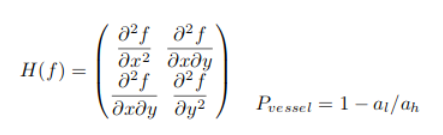
\includegraphics[width=\linewidth]{image/hes.PNG}
	\label{fig:hes}
\end{figure}

\par

Applying this algorithm in our experimentation to a single layer alone we found the results to be quite noisy, as shown Figure  \ref{fig:fig1}, though through visual inspection we could see vessel pixels correctly being identified. Attila Budai, Ruediger Bock, Andreas Maier, Joachim Hornegger, Georg Michelson's paper "Robust Vessel Segmentation in Fundus Images" \cite{22}, of which Budai and Michelson share authorship with the first paper, describes a similar but more robust implementation.

\begin{figure}[H]
	\centering
	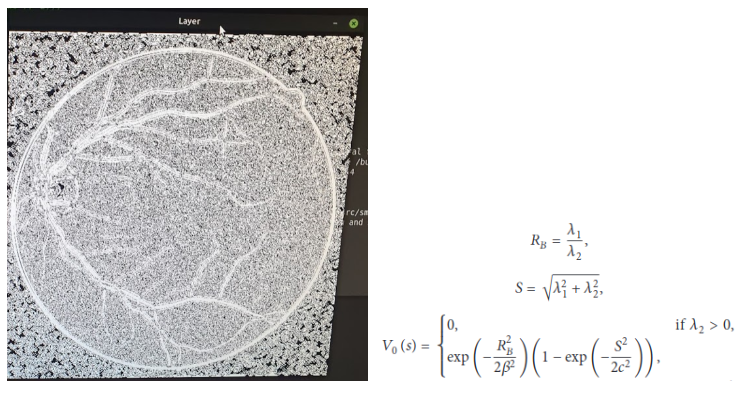
\includegraphics[width=\linewidth]{image/fig1.PNG}
	\caption{Segmentation output without resolution hierarchy}
	\label{fig:fig1}
\end{figure}

\par

In addition to a different "vesselness" function for calculating the value of each pixel on the output layer, pre-processing and post-processing steps are described. For pre-processing, histogram stretching and bilateral filtering was applied to the input layer to provide a larger contrast of colours for the algorithm to process, and to smooth out noise that could create potential false positives for vessel detection. After creation of each output layer, morphological post processing was conducted to fill gaps in the vessels and thin them out, and again after image combination to increase accuracy.


\subsection{Methodology}
\label{ssec:gmethod}

The pipeline of our approach is defined in Fig \ref{fig:gaussian} The processes are classified into pre-processing, vesselness extraction and post-processing which are explained below.

\begin{figure*}[t]
	\centering
	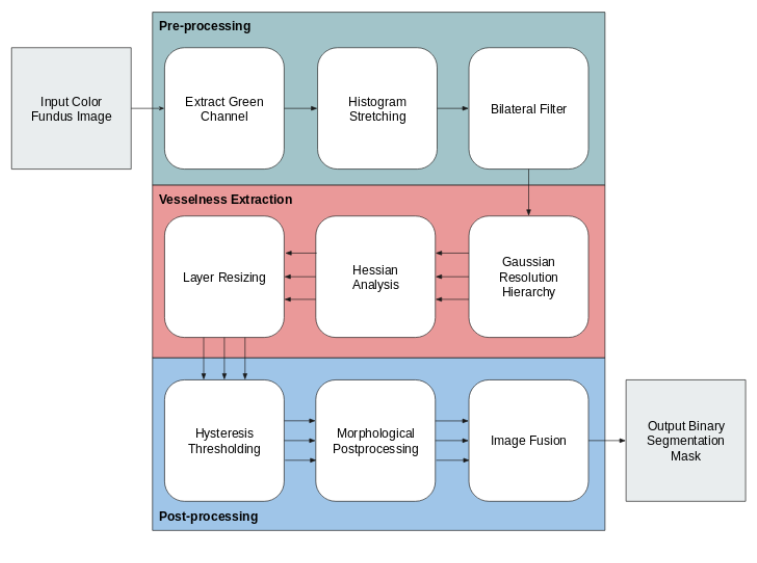
\includegraphics[scale=0.7]{image/gaussian.PNG}
	\caption{Gaussian Pyramid Pipeline Overview}
	\label{fig:gaussian}
\end{figure*}

\subsubsection{Image preprocessing}
\label{sssec:gpreprocess}
\par
The input images for this experiment are digital color fundus photographs. Our analysis are restricted to green channel as this offers the highest contrast between vessels and background. Histogram stretching is performed on the green channel to increase contrast helping the algorithm to detect small changes. Further bilateral filtering is applied to denoise the image by smoothing intensity changes while preserving the boundaries.


\subsubsection{Vesselness Extraction}
\label{sssec:vessel}

\par
Hessian analysis is performed on 3x3 windows and Hessian matrix is calculated for the neighbourhood window of each pixel. The eigenvalues of the Hessian matrix are calculated which signifies the lowest and highest curvature in the neighbourhood. The vesselness feature of the center pixel is calculated applying Frangi’s formula.
\par
The hessian analysis is applied on all layers in the resolution hierarchy. The outputs are resized to the original image size before pipelining them to post processing.

\subsubsection{Image post-processing}
\label{sssec:post}

\par
After performing Vesselness Extraction, the resized image from each of the Gaussian Resolution Hierarchy layer is resized to the original image’s size. We perform a thresholding technique, called Hysteresis thresholding proposed by Canny \cite{23}. The hysteresis method uses two thresholding values to binarize the image unlike a simple thresholding method. The first threshold value, which is the higher of the two, is used to determine high contrast parts of the image. All pixels above the first threshold value is labeled as vessel pixels. Pixels between first and second threshold values are considered as vessel pixels only if it’s connected in the image to a pixel labeled as vessel pixel by the higher threshold value. Hysteresis thresholding thus achieves better results when the fundus image has areas of low contrast where it’s normally difficult using a simple thresholding to differentiate between vessel and noise. The thresholding has been performed using different values of thresholds for each layer.
\par
Then we perform morphological operations, thinning and morphological closing on all the gaussian pyramid layers. Thinning is done to account for over segmentation of thin vessels caused usually in higher layers. So this operation is selectively applied only on higher layers. Morphological closing smoothens the boundaries and small gaps inside the vessels are filled while removing unwanted images.
\par
The final segmented image is obtained by doing a bitwise OR operation on the thresholded image for all resolution hierarchy. Vessel detected in one of the resolution hierarchy therefore will appear in the final output.

\subsection{Experimental Setup}
\label{ssec:gsetup}
\par

Initial experimentation of Hessian analysis on the raw original images resulted in noisy segmentation. Preprocessing input images using histogram stretching and bilateral filtering helped by increasing contrast and reducing noise while preserving edges. Images in Fig \ref{fig:3}, \ref{fig:4} and \ref{fig:5}.
\par

\begin{figure}[H]
	\centering
	\includegraphics[scale=0.7]{image/3.png}
	\caption{Original image}
	\label{fig:3}
\end{figure}

\begin{figure}[H]
	\centering
	\includegraphics[scale=0.7]{image/4.png}
	\caption{Histogram Stretching}
	\label{fig:4}
\end{figure}

\begin{figure}[H]
	\centering
	\includegraphics[scale=0.7]{image/5.png}
	\caption{Bilateral Filter}
	\label{fig:5}
\end{figure}


Hessian analysis was done on 3x3 neighbourhoods in each of the resolution hierarchy layers. The effectiveness of our method relied on finding the right values for the constants in the Frangi’s formula. We found that running analysis of all resolution hierarchy layers did not produce the best results. So unique values were used for each layers so that the larger layers in the pyramid captures more information while smaller layers capture the thicker vessels with more accuracy.
\par
The idea of using different parameters for the layers also improved our hysteresis thresholding. After carefully tweaking we found the values in the table giving us the best results. Finding good values required some manual observation of output images from each resolution hierarchy layers. The values we used are given in Table \ref{table:2}.

\begin{table*}[t]
\centering
 \begin{tabular}{|c| c c c|} 
 \hline
 Thresholds & Highest hierarchy & Second hierarchy & Lowest hierarchy\\ [0.5ex] 
 \hline
 First threshold & 30 & 50 & 30 \\ 
 \hline
 Second threshold & 70 & 100 & 70\\
 \hline
\end{tabular}
\vspace*{0.25cm}
\caption{Hysteresis Thresholding values}
\label{table:2}
\end{table*}

\par

After combining the information found from all resolution hierarchy layers, a final morphological closing operation performed removed some of the gaps inside the segmented vessels.

\subsection{Evaluation and Results}
\label{ssec:gresults}
\par

The metrics obtained on running on 20 images are shown in Table \ref{table:3}. The manual segmentation provided were used as the ground truth to calculate true positives, true negatives, false positives, and false negatives.

\begin{table}[H]
\centering
 \begin{tabular}{|c| c|} 
 \hline
 Accuracy & 87.49\\ [0.5ex] 
 \hline
 Sensitivity & 52.43 \\ 
 \hline
 Specificity & 90.8\\
 \hline
\end{tabular}
\vspace*{0.25cm}
\caption{Accuracy metrics}
\label{table:3}
\end{table}

\subsection{Conclusion and future works}
\par

A multiresolution method was implemented for segmenting blood vessels in fundus photographs. The method offers good accuracy and sensitivity with reduced computational complexities.
\par
Accuracy gains with the method because lower resolution images could capture thick vessels better. The computational demands were reduced as a 3x3 window could be effectively used with resolution hierarchy.
\par
Future works involves reducing false positives by doing Specular Reflex Correction to account for bright specular reflex caused by camera flash in some fundus photographs. Tweaking the kernel for morphological post processing can further reduce noise.

\bibliographystyle{IEEEtran}
\bibliography{references}


% that's all folks
\end{document}


